The central quantity in Bayesian statistics is the posterior distribution $p(z|x)$.
However, in many
nontrivial probabilistic models, including our own, the posterior distribution is intractable to calculate.
Calculation of the posterior requires us to compute the marginal likelihood, $p(x)$, which involves integrating over the latent variable $z$. 
In our model, the latent variable space is high dimensional: it is the set of all catalogs. Approximate methods such as MCMC and variational inference are therefore required. 

Variational inference~\cite{Blei_2017_vi_review, Jordan_intro_vi, Wainwrite_graph_models_vi} posits a family of distributions $\mathcal{Q}$ and seeks
the distribution $q^*\in \mathcal{Q}$ that is closest to the exact posterior
in $\KL$ divergence. 
$\mathcal{Q}$ is chosen such that $q^*$ will not be too difficult to find via optimization. 
We index the distributions in $\mathcal{Q}$ using a real-valued vector $\eta$, then seek $\eta^*$ satisfying
\begin{align}
   \eta^* &= \argmin_{\eta} \mathrm{KL}\Big[\,q_\eta(z | x)\, \| \,p(z | x)\,\Big].
   \label{eq:kl_objective}
\end{align}

Minimizing the $\KL$ divergence in~\eqref{eq:kl_objective} is equivalent to maximizing the evidence lower bound (ELBO)~\cite{Blei_2017_vi_review}:
\begin{align}
    \mathcal{L}_{elbo}(\eta) = 
    \Expect_{q_\eta(z | x)}\Big[\log p(x, z) - \log q_\eta(z | x)\Big].
    \label{eq:elbo}
\end{align}
Computing the ELBO does not require computing the marginal distribution $p(x)$, which is intractable, or the posterior distribution $p(z | x)$, which would be circular. 

\subsection{The variational distribution}
\label{sec:var_distr}
% We now describe our family of distributions $\mathcal{Q}$. 
Traditionally in variational inference, the posterior approximation $q_\eta$ depends on the data $x$ only implicitly, 
in that $\eta^*$ is chosen according to~\eqref{eq:kl_objective}.
In this case, $q_\eta(z | x)$ is usually written $q_\eta(z)$, suppressing the dependence on $x$.

The generative model in Section~\ref{sec:gen_model} does not assume any hierarchical structure over replicated  images. Therefore, given a new image $x^{new}$, the posterior factorizes; in other words,
$p(z^{new}, z | x^{new}, x) = p(z^{new} | x^{new}) p(z | x)$. 
To find a variational  approximation to the posterior $p(z^{new} | x^{new})$, the optimization problem~\eqref{eq:kl_objective} must be solved again with $x = x^{new}$.
Even in models with hierarchical structure, the variational distribution will generally need to be updated via optimization for every newly observed data point. 

On the other hand, 
in {\itshape amortized} variational
inference~\cite{kingma2013autoencoding, rezende2014stochastic}, $q_\eta$ explicitly depends on the data. 
A flexible, parameterized function maps input $x$, in this case an observed image, to the parameters of a variational distribution on the latent space $\mathcal{Z}$. 
Typically, the function is a neural network, in which case the variational parameters $\eta$ are the neural network weights. 
After the neural network is fitted with~\eqref{eq:kl_objective} using a collection of observed $x$'s, the approximate posterior $q_\eta(z^{new} | x^{new})$ for a new data point 
$x^{new}$ can be evaluated with a single forward pass through the neural network. 
No additional run of an iterative optimization routine is needed for a new data point $x^{new}$. 


The following subsections detail the construction of our variational distribution. 

\subsubsection{The factorization}
\label{sec:factorization}
To make the objective in \eqref{eq:kl_objective} tractable, the family $\mathcal{Q}$ is normally restricted to probability distributions 
without conditional dependencies between some latent variables. In the most extreme case, known as mean-field variational inference, the variational distribution completely factorizes across all latent variables. 

Our factorization instead has a spatial structure. 
First, we partition the full $H \times W$ image into disjoint $R \times R$ tiles. 
$R$ will be chosen such that the probability of having three or more stars in one tile is small. 
In this way, the cataloging problem decomposes to inferring only a few stars at a time (Section~\ref{sec:nn_archetecture}). 

Let $S = \sfrac{H}{R}$ and $T = \sfrac{W}{R}$ and assume without loss of generality that $H$ and $W$ are multiples of $R$.
For $s = 1, ..., S$ and $t = 1, ..., T$,
the tile $\tilde x_{st}$ is composed of the following pixels:
\begin{align}
    \tilde x_{st} = \{x_{hw} : Rs \leq h \leq R(s+1) \text{ and } Rt \leq w \leq R(t+1)\}.
    \label{eq:tiles}
\end{align}
Figure~\ref{fig:ex_tiles} gives an example with $R = 2$. 
\begin{figure}[!h]
    \centering
    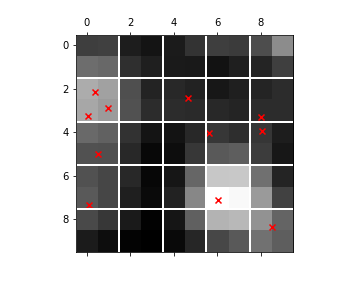
\includegraphics[width = 0.5\textwidth]{figures/vi_figures/example_tiled.png}
    \vspace{-1cm}
    \caption{Tiling a $10 \times 10$ pixel image into $2 \times 2$ tiles.}
    \label{fig:ex_tiles}
\end{figure}

Let $\tilde N^{(s, t)}$ be the number of stars in tile 
$(s,t)$.
Because $\tilde N^{(s, t)}$ is random, 
the cardinality of the set of locations and fluxes in each tile
is also random. 
To handle the trans-dimensional parameter space, 
we consider a {\itshape triangular array} of latent variables
on each tile:
\begin{align}
    \tilde\ell^{(s, t)} &= (\tilde\ell_{N, i}^{(s, t)} : i = 1, ..., N; N = 1, 2, ...); \\
    \tilde f^{(s, t)} &= (\tilde f_{N, i}^{(s, t)} : i = 1, ..., N; N = 1, 2, ...),
\end{align}
where $\tilde\ell_{N, i}^{(s, t)}$ and $\tilde f_{N, i}^{(s, t)}$ are the elements of the triangular array corresponding to location and fluxes, respectively. 

Tile locations $\tilde\ell_{N, i}^{(s, t)} \in [0, R]\times[0, R]$ give the location of stars within a tile. The fluxes $\tilde f_{N, i}^{(s, t)}$ are vectors in $\mathbb{R}^B_+$ (one flux for each band). 

Call $(\tilde N^{(s, t)}, \tilde \ell^{(s, t)}, \tilde f^{(s, t)})_{s=1,t=1}^{S,T}$ the {\itshape tile latent variables}; 
succinctly denote tile latent variables as $\tilde z$. 
The ultimate latent variable of interest is $z = \{N, (\ell_i, f_{i,1}, ..., f_{i,B})_{i = 1}^N\}$, the catalog for the full image. 
A distribution on $z$ is obtained by first constructing a mapping from $\tilde z$ to $z$.
We then define a distribution 
on the tile latent variables $\tilde z$, which in turn  induces 
a distribution on $z$.  


We now detail the mapping $\tilde z\mapsto z$ (see Figure~\ref{fig:tile_to_full_schm} for a schematic).  
The number of stars in the catalog is 
\begin{align}
    N = \sum_{s=1}^{S}\sum_{t=1}^T \tilde N^{(s, t)}. 
\end{align}
For every tile $(s,t)$, we index into the $\tilde N^{(s,t)}$-th
row of the triangular array of tile latent variables:
the fluxes in the catalog are
\begin{align}
    \{f_i\}_{i=1}^N = \Big\{\tilde f_{\tilde N^{(s, t)}, i}^{(s, t)} : i = 1, ..., \tilde N^{(s, t)}, s = 1, ..., S, t = 1, ..., T \Big\},
\end{align}
and the corresponding locations are
\begin{align}
    \{\ell_i\}_{i = 1}^N = \left\{\tilde \ell_{N^{(s, t)}, i}^{(s, t)} + 
    \begin{pmatrix}
    Rs \\ Rt
    \end{pmatrix} 
    : i = 1, ..., N^{(s, t)}, s = 1, ..., S, t = 1, ..., T\right\}. 
\end{align}
The tile location is shifted by $(Rs, Rt)$ to obtain the location in the full image. 

Given this mapping from tile latent variables to the catalog of interest, 
\begin{align}
 \big(\tilde N^{(s, t)}, \tilde \ell^{(s, t)}, \tilde f^{(s, t)}\big)_{s=1, t = 1}^{S, T}
\mapsto     
\{N, (\ell_i, f_{i,1}, ..., f_{i,B})_{i = 1}^N\},
\label{eq:patch_to_full_map}
\end{align}
a distribution on the tile latent variables induces a distribution on catalogs. 

Our variational distribution on $\tilde z$ factorizes over image tiles:
\begin{align}
    \tilde q_\eta\big( \big(\tilde N^{(s, t)}, \tilde \ell^{(s, t)}, \tilde f^{(s, t)}\big)_{s=1, t = 1}^{S, T}|x\big) 
    &=
    \prod_{s = 1}^S \prod_{t=1}^T
    \tilde q_\eta\big(\tilde N^{(s, t)}, \tilde \ell^{(s, t)}, \tilde f^{(s, t)} | x\big).
    \label{eq:factorize_patches}
\end{align}
Within each tile $(s,t)$, the distribution also fully factorizes: 
\begin{align}
    \tilde q_\eta\big(\tilde N^{(s, t)}, \tilde \ell^{(s, t)}, \tilde f^{(s, t)} | x\big)
    &= 
    \tilde q_\eta\big(\tilde N^{(s, t)} | x\big)
    \prod_{n = 1}^\infty \prod_{i = 1}^n 
    \tilde q_\eta\big(\tilde \ell_{n,i}^{(s, t)} | x\big)
    \tilde q_\eta\big(\tilde f_{n,i}^{(s, t)} | x\big).
    \label{eq:factorize_within_patch}
\end{align}

If $\tau$ is the mapping in~\eqref{eq:patch_to_full_map}, then the variational distribution on catalogs $z$ is
\begin{align}
    q_\eta(z | x) := \tilde q_\eta(\tau^{-1}(z) | x),
    \label{eq:pull_back_of_q}
\end{align}
where $\tau^{-1}(z)$ is the pre-image of $z$ under $\tau$.


% for the figure
% {\color{blue} \tilde N^{(1,1)} = 2}

% \\

% \\

% \begin{pmatrix}
% (\tilde \ell, \tilde f)_{1, 1} & \\
% \color{blue} (\tilde \ell, \tilde f)_{2, 1} &
% \color{blue} (\tilde \ell, \tilde f)_{2, 2} &
% \end{pmatrix}^{(1,1)}

% \{{\color{Blue} N = 4},
% {\color{red} (\tilde \ell, \tilde f)^{(1,1)}_{2,1},
% (\tilde \ell, \tilde f)^{(1,1)}_{2,2}},
% {\color{DarkGreen} (\tilde \ell, \tilde f)^{(1,2)}_{1, 1}},
% {\color{Orange} (\tilde \ell, \tilde f)^{(2,1)}_{1, 1}}
% \}

\begin{figure}[!tb]
    \centering
    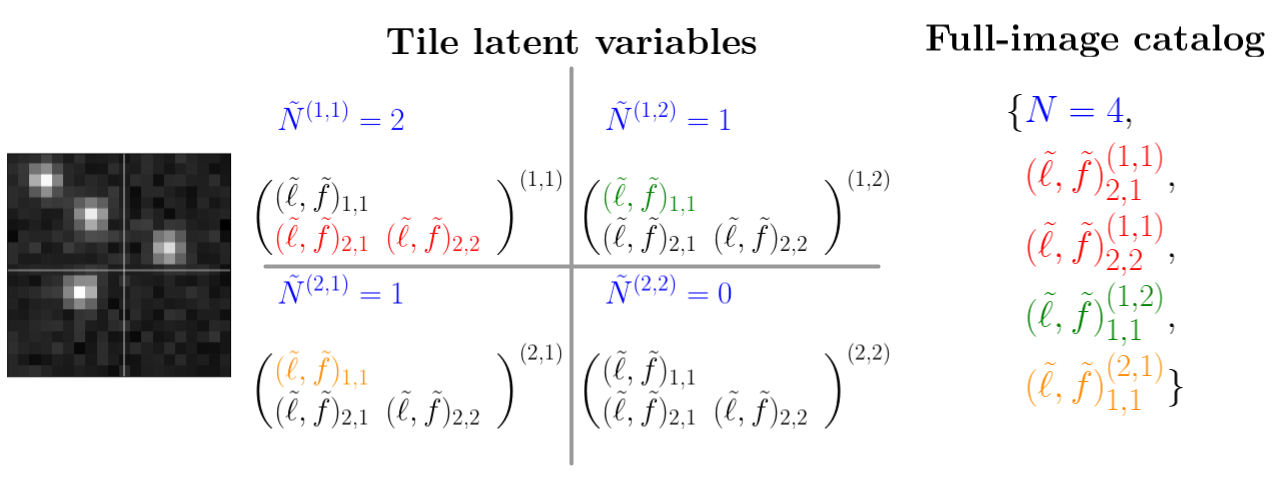
\includegraphics[width = 0.8\textwidth]{figures/vi_figures/tile_to_full_schematic.png}
    \caption{An example image with four tiles illustrating the relationship between tile latent variables and the full-image latent variables. The upper-left tile has two stars; the upper-right and lower-left have one; the bottom right has none. 
    To construct the full-image catalog, we index into the appropriate row of the triangular array on each tile.}
    \label{fig:tile_to_full_schm}
\end{figure}


\noindent{\bf Evaluating the variational distribution}

% \noindent We can use the mapping~\eqref{eq:patch_to_full_map}
% to sample catalogs from our variational distribution.
% If $\tau$ is the mapping in~\eqref{eq:patch_to_full_map}, then 
% we can express the variational distribution
% on the full image catalog $z$ as 
% \begin{align}
%     z &\stackrel{d}{=} \tau\Big( \big(\tilde N^{(s, t)}, \tilde \ell^{(s, t)}, \tilde f^{(s, t)}\big)_{s=1, t = 1}^{S,T}\Big), \notag \\  
%         &\text{where } 
%         \big(\tilde N^{(s, t)}, \tilde \ell^{(s, t)}, \tilde f^{(s, t)}\big)_{s=1, t = 1}^{S,T}
%         \sim 
%         q_\eta\big( \cdot |x\big).
% \end{align}

\noindent Evaluating
the ELBO requires computing the probability of 
$q_\eta(z | x)$
for any given catalog $z = \{N, (\ell_i, f_{i,1}, ..., f_{i,B})_{i = 1}^N\}$. 
By~\eqref{eq:pull_back_of_q}, 
it suffices to evaluate $\tilde q_\eta(\tau^{-1}(z) | x)$. 

Here, $\tau^{-1}(z)$ is a {\itshape set} of tile latent variables because the mapping from tile latent variables to catalogs $z$ is not injective, as we now explain.  

Locations in the catalog $\{\ell_i\}_{i=1}^N$
determine the number of stars on tile $(s,t)$. 
The number of stars $\tilde N^{(s,t)}$ is simply the count of the locations that reside within that tile:
\begin{align}
\tilde N^{(s,t)} = \sum_{i=1}^N 
\mathbf 1 \Big\{\ell_i\in [Rs, R(s+1)] \times [Rt, R(t+1)]\Big\},
\end{align}
where $\mathbf{1}\{\cdot\}$ is the indicator function, equal to one if true and zero if false.

Now, consider $\tilde\ell^{(s, t)}$ and $\tilde f^{(s, t)}$, the triangular array of locations and fluxes on tile $(s,t)$. 
For each $(s,t)$, the $\tilde N^{(s,t)}$-th row 
of the triangular array of fluxes and locations is
determined by the locations and fluxes of stars imaged in tile $(s,t)$; they are determined by the catalog $z$. However, the other rows 
of the triangular arrays are not determined by 
the catalog $z$; they are free to take any value in their domain. Therefore, the mapping $\tau$ is not injective. 

Thus, evaluating the probability of $\tau^{-1}(z)$ under $\tilde q_\eta$ requires marginalizing over the rows of the triangular arrays $\ell^{(s, t)}$ and $\tilde f^{(s, t)}$ that are not determined by $z$. However, 
because $\tilde q_\eta$ fully factorizes, the terms 
in~\eqref{eq:factorize_within_patch} where $n \not= \tilde N^{(s,t)}$ do not enter the
product
after marginalization.
Applying this observation and combining~\eqref{eq:factorize_within_patch} and ~\eqref{eq:factorize_patches}, $\tilde q(\tau^{-1}(z) | x)$ becomes
\begin{align}
    \tilde q(\tau^{-1}(z) | x) = \prod_{s=1}^S\prod_{t=1}^T
    \Big\{
    \tilde q_\eta(\tilde N^{(s,t)} | x) 
    \prod_{i = 1}^{\tilde N^{(s,t)}}
    \tilde q_\eta\big(\tilde \ell_{\tilde N^{(s,t)},i}^{(s, t)} | x\big)
    \tilde q_\eta\big(\tilde f_{\tilde N^{(s,t)},i}^{(s, t)} | x\big)
    \Big\}.
\end{align}
In words, given a catalog $z$,
first convert $z$ to tile random variables;
to compute $q_\eta(z | x)$, it suffices to evaluate $\tilde q_\eta$ only at the rows of triangular 
arrays determined by the number 
of stars falling in each tile. 


% There is a bijection between latent variables on each tile and latent variables on the full image (locations on the full image map to locations on image tiles and vice-versa). 
% \jeff{It's not clear what it means for a latent variable to be ``on a tile''. Why a bijection? They're the same latent variables, right?}
% Thus, a variational distribution for latent variables on tiles induces a variational distribution for latent variables on the full image.
% \jeff{This isn't such a good way to explain it. Better to directly explain the variational distribution over the whole image, from top down, introducing the concept of tiles along the way. Perhaps at the end make the point that our choice of variational distribution does not render the problem embarrassingly parallel.}
% If $\tau$ is the mapping in~\eqref{eq:patch_to_full_map}, then 
% we can express the variational distribution
% on the full image catalog as 
% \begin{align}
%     z &\stackrel{d}{=} \tau\Big( \big(\tilde N^{(s, t)}, \tilde \ell^{(s, t)}, \tilde f^{(s, t)}\big)_{r=1, t = 1}^{s, t}\Big), \notag \\  
%         &\text{where } 
%         \big(\tilde N^{(s, t)}, \tilde \ell^{(s, t)}, \tilde f^{(s, t)}\big)_{r=1, t = 1}^{s, t}
%         \sim 
%         \prod_{r = 1}^R \prod_{t=1}^T q_\eta\big(\tilde N^{(s, t)}, \tilde \ell^{(s, t)}, \tilde f^{(s, t)} | x\big).
% \end{align}
% \jeff{I suggest getting rid of $T$ here. This bijection is a confusing way to explain things. Instead, to refer to the pixels in tile (i, j), you might define
% \[
%     \tilde x_{i,j} = \{x_{hw} : Si \ge h > S(i + 1) \text{ and } Sj \ge w > S(j+1)\}.
% \]
% You could do the same thing for $\tilde f$, etc.
% }
% \jeff{Is there somewhere you say that in the variational distribution, $N = \sum_{k=1}^K N^{(k)}$ ? That might be a good way to put it.}

\subsubsection{Variational distributions on image tiles}
We describe the variational distribution on each tile,
$\tilde q_\eta\big(\tilde N^{(s, t)}, \tilde \ell^{(s, t)}, \tilde f^{(s, t)} | x\big)$. Dropping the index 
$(s,t)$ in this subsection, 
\begin{align}
    \tilde N &\sim \text{Categorical}(
    \omega; 0, ..., N_{max});  \label{eq:var_distr_n}\\
	\tilde \ell_{\tilde N, i} / R &\sim \text{LogitNormal}(\mu_{\ell_{\tilde N, i}}, \text{diag}(\nu_{\ell_{\tilde N, i}}) )\label{eq:var_distr_loc}; \\
	\tilde f^b_{\tilde N, i} &\sim \text{LogNormal}(\mu_{f^b_{\tilde N, i}}, \sigma^2_{f^b_{\tilde N, i}}), \label{eq:var_distr_f}
\end{align}
for $i = 1, ..., \tilde N$; $\tilde{N} = 1, ..., N_{max}$. 
$\omega$ is a $(\tilde N_{max} + 1)$-dimensional vector on the simplex. $\mu_{\ell_{\tilde N, i}}$ and $\nu_{\ell_{\tilde N, }}$ are two-dimensional vectors -- the covariance on locations is diagonal. 
The latent variables also fully factorize within each tile. Note that in the exact posterior, $\tilde N$ has support on the nonnegative integers; in the variational distribution, we truncate at some large $N_{max}$. 


These distributions were taken for convenience: fluxes are positive and right skewed, so we place a normal distribution on log-fluxes; locations are between zero and $R$, so 
we place a normal distribution on the logit of the location scaled by $1 / R$. 

\subsubsection{Neural network architecture}
\label{sec:nn_archetecture}

In each tile, the distributional parameters in \eqref{eq:var_distr_n},
\eqref{eq:var_distr_loc}, and \eqref{eq:var_distr_f} are the output of a neural network. 
The input to the neural network is an $R \times R$ tile, padded with surrounding pixels.
Padding enables the neural network to produce better predictions inside the tile. 
For example, a bright source in the vicinity of but outside the tile will affect the pixel values inside the tile. 
Padding the tiles allows the neural network access to this information. 
The appropriate amount of padding will depend on the PSF width in the analyzed image. 
To catalog the crowded starfield M2 (Section~\ref{sec:results_on_m2}),
we set $R = 2$ and padded the tile with a three-pixel-wide boundary.
Thus, while the distribution on tile latent variables factorize over tiles, the neural network is able to use information from neighboring tiles in producing the distributional parameters. 


Let $\hat x^{(s,t)}$ denote the padded tile pixel intensities (which includes all $B$ bands) and $h_\eta$ be the neural network, which returns the collection of distributional parameters
\begin{align}
    h_\eta(\hat x^{(s,t)}) = (\omega^{(s,t)}, \mu_\ell^{(s,t)}, \nu_{\ell}^{(s,t)}, \mu_f^{(s,t)}, \sigma^{(s,t)}_f).
    \label{eq:nn_output}
\end{align}
The same neural network is evaluated for all tiles $(s,t)$. Our variational parameters are neural network weights, here denoted $\eta$. 
The architecture consists of several convolutional layers followed by a series of fully connected layers (Figure~\ref{fig:starnet_arch}). 
This architecture has been successful on image classification challenges such as ImageNet~\cite{imagenet2015}. 
The optimization of the architecture is left for future work; our focus in this paper is the application of neural networks to provide a variational posterior for cataloging starfields, not the network architecture per se. 


% Convolutional layers are useful for localizing stars, as they make the network invariant to shifts in stellar location. The convolutional kernel in the first layer is $3\times3$ pixels, roughly the full width at half maximum (FWHM) of the PSF. 

\begin{figure}[!tb]
    \centering
    % 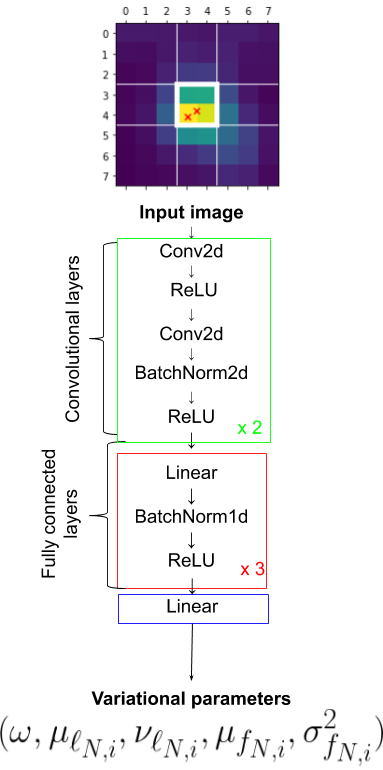
\includegraphics[width=0.4\textwidth]{figures/starnet_archetecture2.png}
    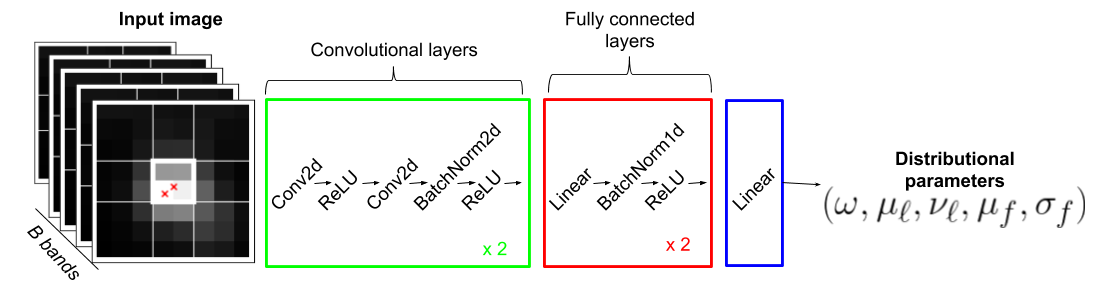
\includegraphics[width=\textwidth]{figures/vi_figures/starnet_archetecture4.png}
    \vspace{-0.5cm}
    \caption{The neural network architecture. For cataloging M2, the input image is an $8\times 8$ padded tile, and the network returns distributional parameters for latent variables contained in the center $2\times 2$ tile.\\
    }
    \label{fig:starnet_arch}
\end{figure}

Note the output dimension of the neural network. For each tile $(s,t)$, the categorical parameter $\omega^{(s,t)}$
lies on the simplex and has dimension $N_{max} + 1$. 
Furthermore, each index of the triangular array
$i = 1, ..., \tilde N^{(s,t)}$, $\tilde N^{(s,t)} = 1, ..., N_{max}$
describes a star. The star has a mean and variance for each location coordinate, and a mean and variance for its flux in each band. 
Thus, for each star $(\tilde N^{(s,t)}, i)$, 
the neural network outputs $2 \times (B + 2)$ parameters. 
In total, the neural network has output dimension $(N_{max} + 1) + (B + 2) \times (N_{max}^2 + N_{max})$. 

% Recall that locations on the 
% full image $\ell_{N, i}$ are parameterized to be in $[0, H] \times [0, W]$. 
% On the tiles, locations $\ell^{(k)}_{N, i}$ are parameterized to be in
% $[0, s] \times [0, s]$. 

Because the output dimension is quadratic in $N_{max}$, factorizing the variational distribution spatially keeps the output dimension of the neural network manageable.
On a crowded starfield with $H = W = 100$, the number of imaged stars is on the order of $10^3$.
If the neural network were to return a variational distribution on the full $100\times 100$ image, the output dimension would be on the order of $(10^3)^2$. 
On the $2\times 2$ tile, we set $N_{max} = 3$, and the output dimension of the neural network with two bands is 53. 
With this factorization, the network can be used for inference on an image of any size. 


We emphasize that while the variational distribution factorizes over $2 \times 2$ tiles, our method does not break the inference problem for the full image into isolated subproblems. The evaluation of the likelihood, e.g., when computing the ELBO in~\eqref{eq:elbo}, is always on the full image. Light from a star within a $2 \times 2$ tile spills over into neighboring tiles, so the likelihood should not and does not decouple across image tiles. 
